% Options for packages loaded elsewhere
\PassOptionsToPackage{unicode}{hyperref}
\PassOptionsToPackage{hyphens}{url}
%
\documentclass[
]{article}
\usepackage{amsmath,amssymb}
\usepackage{iftex}
\ifPDFTeX
  \usepackage[T1]{fontenc}
  \usepackage[utf8]{inputenc}
  \usepackage{textcomp} % provide euro and other symbols
\else % if luatex or xetex
  \usepackage{unicode-math} % this also loads fontspec
  \defaultfontfeatures{Scale=MatchLowercase}
  \defaultfontfeatures[\rmfamily]{Ligatures=TeX,Scale=1}
\fi
\usepackage{lmodern}
\ifPDFTeX\else
  % xetex/luatex font selection
\fi
% Use upquote if available, for straight quotes in verbatim environments
\IfFileExists{upquote.sty}{\usepackage{upquote}}{}
\IfFileExists{microtype.sty}{% use microtype if available
  \usepackage[]{microtype}
  \UseMicrotypeSet[protrusion]{basicmath} % disable protrusion for tt fonts
}{}
\makeatletter
\@ifundefined{KOMAClassName}{% if non-KOMA class
  \IfFileExists{parskip.sty}{%
    \usepackage{parskip}
  }{% else
    \setlength{\parindent}{0pt}
    \setlength{\parskip}{6pt plus 2pt minus 1pt}}
}{% if KOMA class
  \KOMAoptions{parskip=half}}
\makeatother
\usepackage{xcolor}
\usepackage[margin=1in]{geometry}
\usepackage{graphicx}
\makeatletter
\def\maxwidth{\ifdim\Gin@nat@width>\linewidth\linewidth\else\Gin@nat@width\fi}
\def\maxheight{\ifdim\Gin@nat@height>\textheight\textheight\else\Gin@nat@height\fi}
\makeatother
% Scale images if necessary, so that they will not overflow the page
% margins by default, and it is still possible to overwrite the defaults
% using explicit options in \includegraphics[width, height, ...]{}
\setkeys{Gin}{width=\maxwidth,height=\maxheight,keepaspectratio}
% Set default figure placement to htbp
\makeatletter
\def\fps@figure{htbp}
\makeatother
\setlength{\emergencystretch}{3em} % prevent overfull lines
\providecommand{\tightlist}{%
  \setlength{\itemsep}{0pt}\setlength{\parskip}{0pt}}
\setcounter{secnumdepth}{-\maxdimen} % remove section numbering
\usepackage{caption}
\usepackage{booktabs}
\usepackage{longtable}
\usepackage{array}
\usepackage{multirow}
\usepackage{wrapfig}
\usepackage{float}
\usepackage{colortbl}
\usepackage{pdflscape}
\usepackage{tabu}
\usepackage{threeparttable}
\usepackage{threeparttablex}
\usepackage[normalem]{ulem}
\usepackage{makecell}
\usepackage{xcolor}
\ifLuaTeX
  \usepackage{selnolig}  % disable illegal ligatures
\fi
\usepackage{bookmark}
\IfFileExists{xurl.sty}{\usepackage{xurl}}{} % add URL line breaks if available
\urlstyle{same}
\hypersetup{
  pdftitle={Final Report},
  pdfauthor={Olivia Hofmann, Matias Barcelo, and Mike Perkins},
  hidelinks,
  pdfcreator={LaTeX via pandoc}}

\title{Final Report}
\author{Olivia Hofmann, Matias Barcelo, and Mike Perkins}
\date{2024-11-13}

\begin{document}
\maketitle

{
\setcounter{tocdepth}{4}
\tableofcontents
}
\newpage

\section{Problem Description (Business
Understanding)}\label{problem-description-business-understanding}

COVID-19 is a highly contagious respiratory illness that first emerged
in Wuhan, China in December 2019. COVID-19 entered the United States in
January 2020 with the World Health Organization (WHO) declaring COVID-19
a ``global health emergency'' in March 2020. The virus spreads through
respiratory droplets dispersed when someone coughs, sneezes, or even
talks. COVID-19 can cause symptoms including those similar to a cold,
influenza, or pneumonia with the potential to become very severe and
lead to death. The COVID-19 virus overwhelmed healthcare systems and
disrupted economies around the world. {[}1{]} {[}2{]}

The stakeholder for this data analysis is a property developer who is
interested in determining the best location in Texas for developing a
mixed-use building. The stakeholder's key concern is selecting a county
that demonstrates stability and resilience in response to unpredictable
events, like the COVID-19 pandemic. The mixed-use building that the
stakeholder is looking to develop will have space for a gym,
restaurants, pharmacy, and other similar businesses. When deciding where
to build this mixed-use building, the stakeholder is looking for
insights into which counties in Texas have successfully managed public
health crises as situations similar to this would greatly impact the
success of the businesses within his building. Every business that would
be in the mixed-use building would be heavily reliant on consistent
traffic and economic activity. Any change in foot traffic and economic
activity would directly impact the success or failure of each business.
The analysis will include data on COVID-19 cases, COVID-19 deaths, and
the effectiveness of government interventions (such as lock downs and
social distancing). This analysis is crucial for the stakeholder to make
an informed decision regarding this long-term investment, as counties
that respond well to crises are more likely to provide stable
environments for growth and development.

Some questions that the stakeholder would like answered are:

\begin{itemize}
\tightlist
\item
  What are the characteristics of counties in Texas that showed
  resilience during the COVID-19 pandemic, based on COVID-19 case rates?
\item
  What are the economic and social impacts in counties that were more or
  less affected by the pandemic and how might these influence future
  development potential?
\item
  How did COVID-19 impact the workplace and employment rates in the
  various counties?
\item
  Which counties showed consistent consumer foot traffic during the
  pandemic, indicating stable economic activity?
\end{itemize}

All of these questions are critical because the answers will help the
property developer asses the risk and potential returns on his
investment. Data needed to complete this analysis includes COVID-19 data
for the state of Texas, COVID-19 date for the entire United States, and
COVID-19 mobility data for the world. While these datasets seem broad,
each dataset contains necessary features to conduct this analysis, which
will be revealed further in the report. By understanding how different
counties fared during the pandemic, the developer can make an informed
decision regarding where he wants to build, ensuring that the chosen
location offers stability and growth potential, even during unforeseen
circumstances.

\newpage

\section{Income Data in Texas
Counties}\label{income-data-in-texas-counties}

\subsection{Data Collection, Quality, and
Exploration}\label{data-collection-quality-and-exploration}

\subsubsection{Objects to Cluster}\label{objects-to-cluster}

The objects to be clustered in this analysis are the counties in Texas.
To identify which counties demonstrated resilience during the COVID-19
pandemic, income and rent burden metrics will be analyzed alongside
general population data. Some key features for clustering include median
income, income per capita, a couple rent burden levels, and a few income
distribution brackets. These factors provide a comprehensive picture of
each county's economic resilience and ability to maintain stability
during times of crisis.

By examining income distribution and wealth concentration, we can
determine which counties have strong economic foundations. This, in
combination with COVID-19 case and death data, will guide the
stakeholder in making an informed decision on where to invest in
developing a mixed-use building. Counties that managed to sustain
consumer traffic and economic activity during the pandemic will likely
offer more stability and growth potential for future business ventures.

\subsubsection{Features for Clustering}\label{features-for-clustering}

The features analyzed for clustering relate to the category of income
and wealth, which are critical for understanding economic resilience.
These features include income brackets, median income per capita, rent
burden percentages, and population statistics. Each of these features
play a significant role in assessing to what capacity the county can
withstand a widespread challenge such as the COVID-19 pandemic.

\begin{itemize}
\tightlist
\item
  \textbf{Income Levels:} The distribution of households across various
  income levels can provide insight into a county's overall economic
  health and resilience.
\item
  \textbf{Rent Burden:} High rent burden percentages indicate financial
  strain on households, which can affect their ability to manage crises
  effectively.
\item
  \textbf{Median Income and Income per Capita:} These metrics serve as
  broad indicators of wealth within a county. Wealthier counties
  typically have more resources to navigate economic shocks and support
  their communities during difficult times.
\item
  \textbf{Population:} Including population statistics allows for a more
  accurate interpretation of COVID-19 impacts by normalizing the number
  of cases and deaths based on county size.
\end{itemize}

By clustering counties based on these features, we can identify
different income and wealth profiles that may correlate with their
resilience during the pandemic. This analysis will enhance our
understanding of which counties were better equipped to handle the
economic and social disruptions caused by COVID-19, ultimately aiding
the stakeholder in making informed investment decisions.

\subsubsection{Table of Features and Basic
Statistics}\label{table-of-features-and-basic-statistics}

\begingroup\fontsize{10}{12}\selectfont

\begin{longtable}[t]{lrrrr}
\caption{\label{tab:basic statistics}Basic Statistics of Key Features}\\
\toprule
Feature & Mean & SD & Min & Max\\
\midrule
Median Income & 49894.339 & 12132.676 & 24794 & 93645\\
Income per Capita & 24859.020 & 5240.752 & 12543 & 41609\\
Rent > 50\% Income & 2976.004 & 13179.056 & 0 & 158668\\
Rent 30-35\% Income & 1180.870 & 5203.838 & 0 & 61305\\
Income < 10,000 USD & 2469.768 & 8601.256 & 0 & 98715\\
\addlinespace
Income 50,000-59,999 USD & 2945.197 & 10790.454 & 3 & 122390\\
Income 100,000-124,999 USD & 3205.157 & 11657.055 & 0 & 131467\\
Total Population & 107951.228 & 389476.863 & 74 & 4525519\\
\bottomrule
\end{longtable}
\endgroup{}

Because there are a lot of features that represent the wealth and income
category, features were chosen that represent the most critical
dimensions of income distribution and rent burden, while avoiding overly
granular breakdowns. This selection captures the distribution of wealth
(from low to high incomes), general population data, and rent burden,
which are the most relevant features for analyzing the economic
stability of a county.

\begin{itemize}
\tightlist
\item
  \textbf{Median Income:} This gives a central measure of income
  distribution in a county.
\item
  \textbf{Income per Capita:} Shows wealth distribution on a per-person
  basis, which complements median income.
\item
  \textbf{Rent Over 50 Percent:} This is a key indicator of severe rent
  burden, which can signify economic strain in a county.
\item
  \textbf{Rent 30 to 35 Percent:} This provides a threshold of moderate
  rent burden.
\item
  \textbf{Income Less than \$10,000:} Reflects the population in extreme
  poverty, which is crucial for understanding economic vulnerability.
\item
  \textbf{Income \$50,000 - \$59,999:} Represents household earning
  within a middle-income bracket, which can provide insight to stability
  of the county's middle class.
\item
  \textbf{Income \$100,000 - \$124,999:} Indicates a higher income
  range, reflecting the proportion of relatively affluent residents.
\end{itemize}

\subsubsection{Scale of Measurement}\label{scale-of-measurement}

All of the features listed below are ratio scales because they have a
true zero point (e.g., zero income, zero population) and allow for
meaningful arithmetic operations (e.g., calculating differences,
ratios).

\begingroup\fontsize{10}{12}\selectfont

\begin{longtable}[t]{lll}
\caption{\label{tab:scale of measurement}Measurement Scales for Features}\\
\toprule
Feature & Scale & Description\\
\midrule
Median Income & Ratio & Income in USD\\
Income per Capita & Ratio & Per capita income in USD\\
Rent > 50\% Income & Ratio & Households paying >50\% income in rent\\
Rent 30-35\% Income & Ratio & Households paying 30-35\% income in rent\\
Income <10,000 USD & Ratio & Households earning <10,000 USD\\
\addlinespace
Income 50,000-59,999 USD & Ratio & Households earning 50,000-59,999 USD\\
Income 100,000-124,999 USD & Ratio & Households earning 100,000-124,999 USD\\
Total Population & Ratio & Total county population\\
\bottomrule
\end{longtable}
\endgroup{}

\subsubsection{Measures for
Similarity/Distance}\label{measures-for-similaritydistance}

For clustering analysis, various measures of similarity or distance can
be employed based on the features used. The following measures are
particularly relevant:

\begin{itemize}
\tightlist
\item
  \textbf{Euclidean Distance:} This is the most widely used distance
  measure, calculated as the straight-line distance between points in a
  multi-dimensional space. It is especially effective for continuous
  numerical data such as income or population figures, where the
  relationships between data points can be interpreted geometrically.
  Euclidean distance captures the direct linear relationship between
  observations, making it intuitive and straightforward for visualizing
  proximity in clustering contexts. {[}3{]}
\item
  \textbf{Manhattan Distance:} This measure calculates the distance
  between two points by summing the absolute differences of their
  coordinates. Manhattan distance is useful when dealing with outliers
  or when the scale of measurement varies among features. It reflects a
  grid-like path, which can be advantageous in scenarios where a more
  robust metric against extreme values is required. In urban
  environments, for example, it mirrors the layout of streets. {[}4{]}
\item
  \textbf{Standardization/Normalization:} When features exhibit wide
  ranges, normalizing the data before applying distance measures is
  beneficial. This ensures that each feature contributes equally to the
  distance calculation, preventing features with larger scales from
  disproportionately influencing results. {[}5{]}
\end{itemize}

In this analysis, a combination of standardized/normalized distance and
Euclidean distance will be utilized. The data will first be standardized
to ensure that each feature contributes equally to the distance
calculation. The choice of Euclidean distance is justified by its
prevalence and effectiveness for income and population data, which
typically exhibit continuous numerical characteristics. It provides a
clear and meaningful way to measure similarity between counties based on
economic and demographic factors.

\subsubsection{Normalization/Standardization}\label{normalizationstandardization}

Standardization is essential for putting features on a similar scale,
enabling meaningful comparisons across variables and preventing features
with larger ranges or counts from dominating the analysis---especially
in clustering algorithms. Given the wide range of values in the dataset,
it was necessary to standardize the numerical features before proceeding
with clustering or further analysis. The standardization was done using
R and it transforms the data such that each feature has a mean of 0 and
a standard deviation of 1. The county name was not standardized since it
is a categorical variable. Since standardization is applied to numerical
data, this feature was excluded from the process.

\subsection{Modeling and Evaluation}\label{modeling-and-evaluation}

\subsubsection{K-Means Clustering}\label{k-means-clustering}

The K-Means clustering plot shows how Texas counties are grouped into
two distinct clusters (1 and 2). Each point on the plot represents a
county, and the clusters are visualized using different shapes and
colors. The boarder around each cluster provides a visual boundary for
each group. This clustering helps uncover patterns among the counties
based on their economic resilience during the COVID-19 pandemic.

\vspace{10pt}

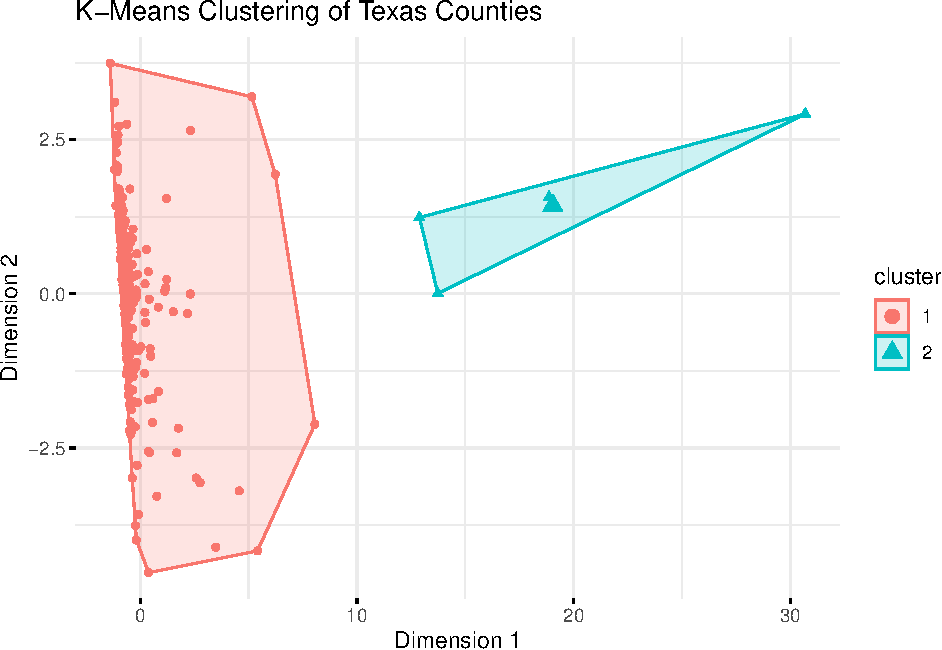
\includegraphics{Final-Report_files/figure-latex/k-means clustering-1.pdf}

\captionof{figure}{K-Means Clustering of Texas Counties}

\vspace{10pt}

A summary statistics table is used to provide a detailed breakdown of
the average values for key features across the two clusters identified
through K-Means clustering. Each cluster represents a distinct group of
Texas counties with similar economic, demographic, and pandemic
characteristics. The table displays the average median income, income
per capita, rent burden levels (both for households spending more than
50\% and 30-35\% of their income on rent), confirmed COVID-19 cases,
deaths, and total population for each cluster.

\begin{table}[!h]
\centering
\caption{\label{tab:k-means summary statistics by cluster}Summary Statistics by Cluster}
\centering
\fontsize{7}{9}\selectfont
\begin{tabular}[t]{>{\raggedright\arraybackslash}p{1.5cm}>{\raggedleft\arraybackslash}p{1.5cm}>{\raggedleft\arraybackslash}p{1.5cm}>{\raggedleft\arraybackslash}p{1.5cm}>{\raggedleft\arraybackslash}p{1.5cm}>{\raggedleft\arraybackslash}p{1.5cm}>{\raggedleft\arraybackslash}p{1.5cm}r}
\toprule
cluster & Avg
Median
Income & Avg
Income
per Capita & Avg
Rent
> 50\% & Avg
Rent
30-35\% & Avg
Confirmed
Cases & Avg
Deaths & Total
Population\\
\midrule
1 & 49780.86 & 24786.04 & 1551.7 & 615.408 & 5078.896 & 89.052 & 65864.8\\
2 & 56987.00 & 29420.25 & 91995.0 & 36522.250 & 217182.500 & 2529.000 & 2738352.8\\
\bottomrule
\end{tabular}
\end{table}

Cluster 1 has a high concentration of points while Cluster 2 captures a
much smaller group. This incredibly uneven distribution suggests the
clustering is not a great representation of the counties.

\vspace{5pt}

\begin{itemize}
\tightlist
\item
  \textbf{Average Median Income:} Cluster 1 had an average median income
  of 47,780.86 USD and Cluster 2 had an average median income of
  56,987.00 USD. This shows a very moderate income difference of less
  than 10,000 USD.
\item
  \textbf{Average Deaths:} This is a pretty big discrepancy as Cluster 2
  experiences 2,529 average deaths while Cluster 1 only experienced 89.
  This indicates that Cluster 2 captures a very specific subset of
  counties with higher COVID-19 mortality.
\end{itemize}

\vspace{5pt}

This clustering does not offer a clear, interpretable division aligned
with economic or pandemic impact metrics, as variation between clusters
in largely skewed. This unsupervised K-Means clustering could perform
better with supervision.

\paragraph{Suitable Number of
Clusters}\label{suitable-number-of-clusters}

The Elbow Method plots the WSS (Within-Cluster Sum of Squares) for
different number of clusters. WSS measures how tightly the data points
are grouped around the centroids of the clusters. After a certain point,
adding more clusters provides diminishing returns, meaning the reduction
in WSS becomes negligible. The optimal number of clusters is found at
the ``elbow'' point, where the rate of decrease in WSS sharply levels
off. In the following elbow plot, the elbow occurs around 2 clusters.

\vspace{10pt}

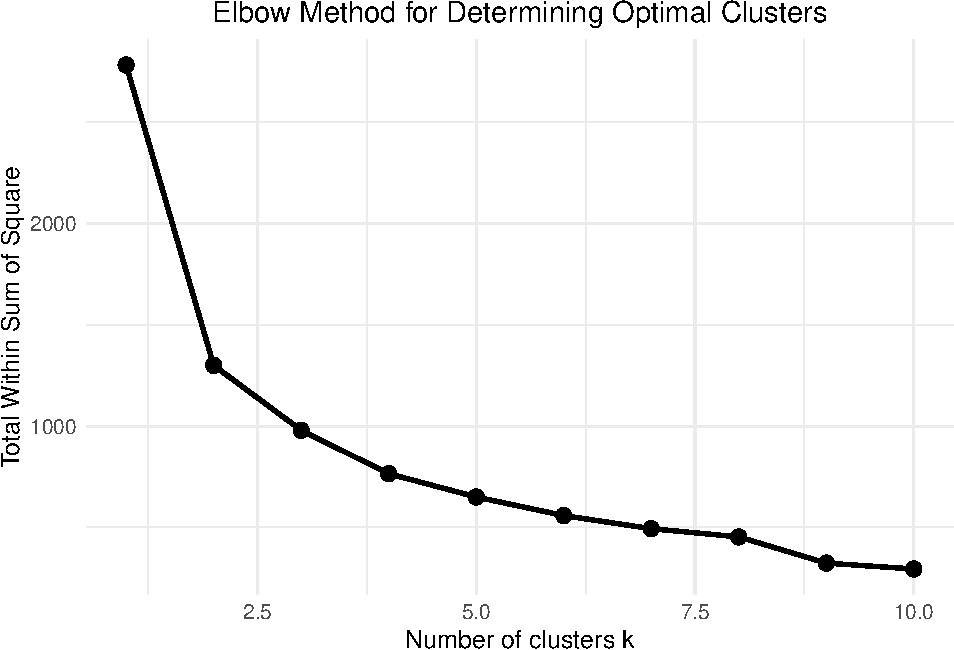
\includegraphics{Final-Report_files/figure-latex/k-means optimal cluster-1.pdf}

\captionof{figure}{Elbow Method for Determining Optimal Clusters}

\vspace{10pt}

The Silhouette Method evaluates how well each data point fits within its
assigned cluster compared to other clusters. The Silhouette score ranges
from -1 to 1, with values close to 1 meaning that the points are
well-clustered. In the following Silhouette chart, the peak occurs at 2
clusters.

\vspace{10pt}

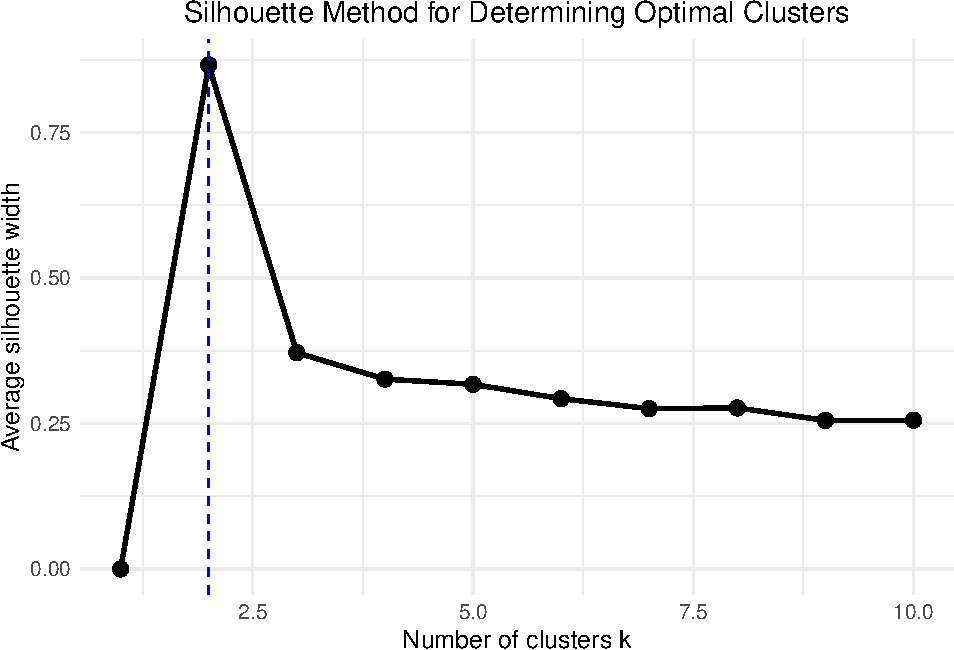
\includegraphics{Final-Report_files/figure-latex/k-means optimal cluster silhouette-1.pdf}

\captionof{figure}{Silhouette Method for Determining Optimal Clusters}

\vspace{10pt}

After considering both of these models, it was decided to do 2 clusters.
Because of the consistency across both methods, 2 clusters was the clear
choice.

\paragraph{Unsupervised Evaluation}\label{unsupervised-evaluation}

A silhouette plot is used as the unsupervised evaluation to assess the
quality and cohesion of clusters generated by the K-Means algorithm. The
silhouette width is a metric used to evaluate how well each data point
fits within its assigned cluster relative to other clusters. Values near
1 indicate that data points are well-matched to their own cluster and
poorly matched to neighboring clusters (high-quality clustering). Values
near 0 suggest that the data points lie equally far from two neighboring
clusters (uncertainty in clustering assignments).

\vspace{10pt}

\begin{verbatim}
##   cluster size ave.sil.width
## 1       1  250          0.87
## 2       2    4          0.45
\end{verbatim}

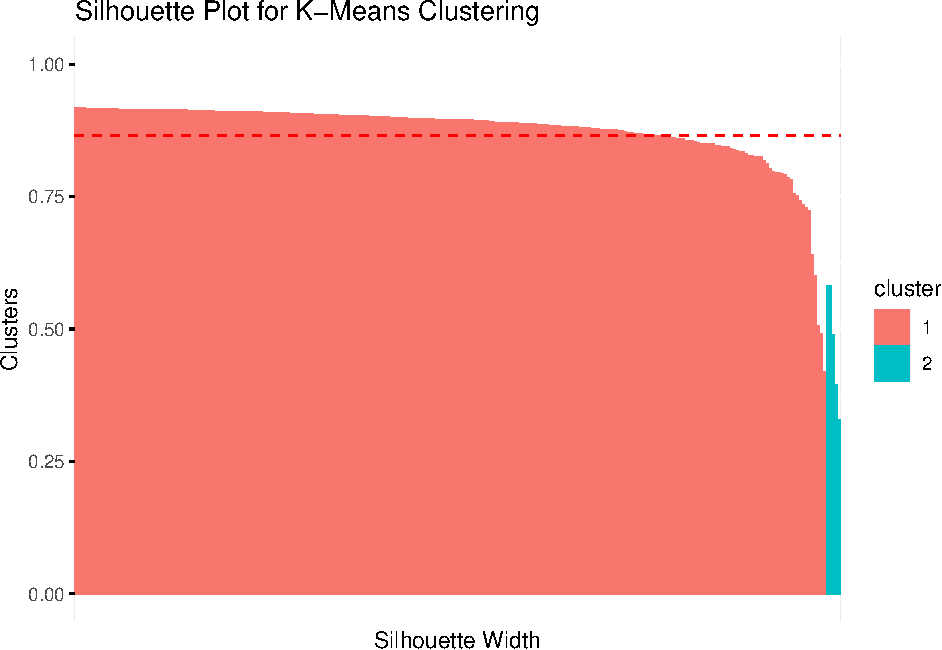
\includegraphics{Final-Report_files/figure-latex/heirarchical silhouette plot-1.pdf}

\captionof{figure}{Silhouette Plot for K-Means Clustering}

\vspace{10pt}

\begin{itemize}
\tightlist
\item
  \textbf{Cluster 1 (Red):} The size of this cluster is 250 points with
  an average silhouette width of 0.87. This can be interpreted to mean
  that most of the data points are well-separated from other clusters
  and they have a high degree of cohesion. Cluster 1 can be defined as
  compact and well-defined within the data.
\item
  \textbf{Cluster 2 (Blue):} The size of this cluster is 4 points with
  an average silhouette width of 0.45. This can be interpreted to mean
  that the points within the cluster are less cohesive and lack a clear
  grouping, leading to a weaker clustering group.
\end{itemize}

\paragraph{Ground Truth Feature}\label{ground-truth-feature}

The feature used for the ground truth features is the COVID-19 deaths,
comparing the clusters to the death-to-case ratio category (Lower:
\textless0.025, Higher: \textgreater0.025). The motivation for choosing
this feature as the ground truth feature stems from the goal of
examining how wealth and economic conditions impacted the pandemic
outcomes.

\vspace{5pt}

\begin{itemize}
\tightlist
\item
  The analysis seeks to determine if wealthier counties, indentified
  through income-realted clustering, exhibit better pandemic performance
  measured through lower mortality rates relative to confirmed cases.
\item
  By using ``Lower'' and ``Higher'' categories, the analysis is
  simplfied, making it easier to interpret and compare income groups.
  Additionally, to truly show a comparison between unsupervised and
  supervised clustering, it was decided to stay consistent with 2
  clustering groups.
\item
  Mortality rates serve as a crutial public health indicator, directly
  reflecting the severity of the pandemic's impact on a county. This
  feature can provide meaningful insight into how income of a county can
  indicate resilience and lower mortality rates for a pandemic like
  COVID-19.
\end{itemize}

\vspace{5pt}

The choice of this feature thus helps explore the correlation between
economic factors and the severity of the pandemic's impact, offering
critical and clear insights into the resilience and vulnerabilities of
different counties.

\vspace{10pt}

\begin{verbatim}
##    
##     Lower Higher
##   1   145    105
##   2     4      0
\end{verbatim}

\captionof{figure}{Ground Truth Cluster Comparison}

\vspace{10pt}

\paragraph{Supervised Evaluation}\label{supervised-evaluation}

The K-Means clustering plot shows how Texas counties are grouped into
two distinct clusters (1 and 2). The features used for clustering are
the death\_case\_ratio (the ratio of COVID-19 deaths to confirmed cases)
and income\_per\_capita. The features were scaled to have a mean of zero
and standard deviation of one, making sure that both features contribute
equally to the clustering process. The difference between this
clustering and the previous K-Means clustering is that this is
supervised, meaning that the x and y axis are intentionally chosen to
provide a simplified and clear result. The clusters represent groups of
counties that share similar characteristics in terms of economic
conditions and pandemic impact. Counties within each cluster exhibit
more similarity to each other than to those in the other cluster.

\vspace{10pt}

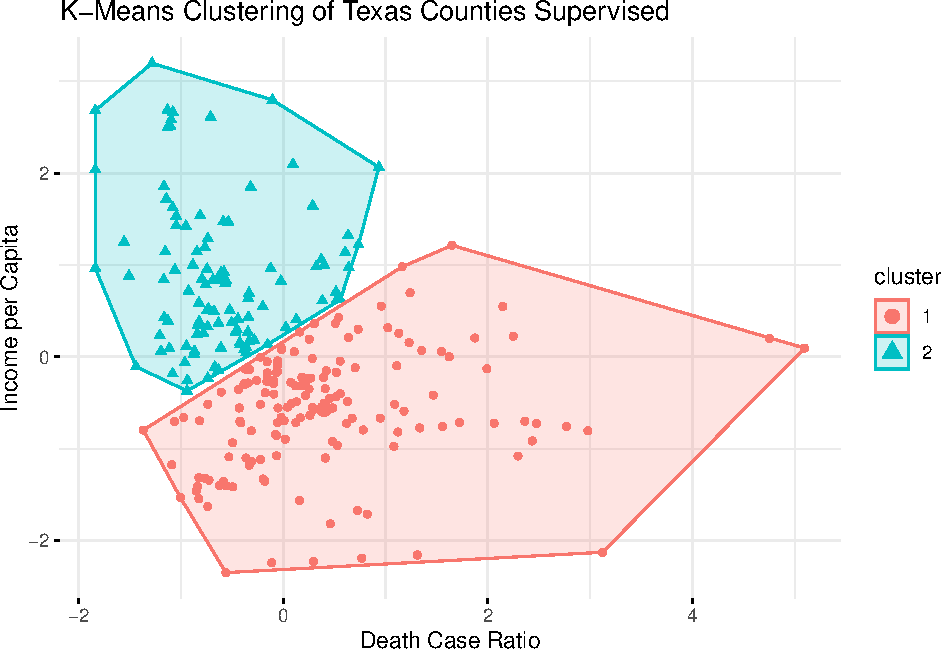
\includegraphics{Final-Report_files/figure-latex/k-means clustering supervised-1.pdf}

\captionof{figure}{K-Means Clustering of Texas Counties Supervised}

\vspace{10pt}

A summary statistics table, similar to the previous clustering method,
is used to provide a detailed breakdown of the average values for key
features across the two supervised clusters identified through K-Means
clustering. Each cluster represents a distinct group of Texas counties
with more similar economic, demographic, and pandemic characteristics.
The table displays the average median income, income per capita, rent
burden levels (both for households spending more than 50\% and 30-35\%
of their income on rent), confirmed COVID-19 cases, deaths, and total
population for each cluster.

\begin{table}[!h]
\centering
\caption{\label{tab:supervised k-means summary statistics by cluster}Summary Statistics by Cluster}
\centering
\fontsize{7}{9}\selectfont
\begin{tabular}[t]{>{\raggedright\arraybackslash}p{1.25 cm}>{\raggedleft\arraybackslash}p{1.25 cm}>{\raggedleft\arraybackslash}p{1.25 cm}>{\raggedleft\arraybackslash}p{1.25 cm}>{\raggedleft\arraybackslash}p{1.25 cm}>{\raggedleft\arraybackslash}p{1.25 cm}>{\raggedleft\arraybackslash}p{1.25 cm}>{\raggedleft\arraybackslash}p{1.25 cm}r}
\toprule
cluster & Avg
Median
Income & Avg
Income
per Capita & Avg
Rent
> 50\% & Avg
Rent
30-35\% & Avg
Confirmed
Cases & Avg
Deaths & Avg
Death Case Ratio & Total
Population\\
\midrule
1 & 43937.72 & 21876.61 & 804.7255 & 297.6667 & 3309.477 & 80.98693 & 0.0300654 & 37969.71\\
2 & 58917.73 & 29376.93 & 6265.1683 & 2518.7921 & 16159.446 & 197.90099 & 0.0165567 & 213962.83\\
\bottomrule
\end{tabular}
\end{table}

\vspace{5pt}

This clustering uses interpretable features: death case ratio and income
per capita. This makes the clusters more meaningful, reflecting the
economic status directly. The data is more evenly distributed between
the two clusters, providing a clearer separation of counties. Clusters 1
and 2 have a relatively even distribution of points, suggesting that the
clustering is a good representation of the counties.

\vspace{5pt}

\begin{itemize}
\tightlist
\item
  \textbf{Average Median Income:} Cluster 1 had an average median income
  of 58,917.73 USD and Cluster 2 had an average median income of
  43,937.72 USD. This shows a very clear differentiation in economic
  status. The different is around 15,000 USD.
\item
  \textbf{Average Death Case Ratio:} Cluster 1 has an average ratio of
  0.0166 which is significantly lower than Cluster 2's average ratio of
  0.0301. This highlights the relationship between economic conditions
  and pandemic outcomes more effectively.
\end{itemize}

\vspace{5pt}

The two K-Means clustering analyses (supervised and unsupervised) aim to
categorize Texas counties based on economic and pandemic-related
features, but they differ significantly in terms of clarity, precision,
and interpretability.

\vspace{5pt}

Within Clusters 1 and 2, the counties are grouped based on their income
and rent burdens. There are three income groups (Low: Income per Capita
\textless{} 25,000 USD, Middle: 25,000 USD \textless= Income per Capita
\textless{} 40,000 USD, High: Income per Capita \textgreater{} 40,000
USD) and two rent burden groups (Low: Rent over 50 Percent \textless=
5000, High: Rent over 50 Percent \textgreater{} 5000) that are used to
provide more detailed comparison of the clusters.

\begin{table}[!h]
\centering
\caption{\label{tab:supervised grouping}Summary Statistics by Subgroups Within Clusters}
\centering
\fontsize{7}{9}\selectfont
\begin{tabular}[t]{>{\raggedright\arraybackslash}p{1.25 cm}>{\raggedright\arraybackslash}p{1.25 cm}>{\raggedright\arraybackslash}p{1.25 cm}>{\raggedleft\arraybackslash}p{1.25 cm}>{\raggedleft\arraybackslash}p{1.25 cm}>{\raggedleft\arraybackslash}p{1.25 cm}>{\raggedleft\arraybackslash}p{1.25 cm}>{}p{1.25 cm}}
\toprule
cluster & income\_group & rent\_burden\_group & Avg Median Income & Avg Income per Capita & Avg Death Case Ratio & Total Population\\
\midrule
1 & Low Income & High Rent Burden & 39219.50 & 17058.50 & 0.0257519 & 591047.25\\
1 & Low Income & Low Rent Burden & 43140.55 & 21125.65 & 0.0279399 & 23914.66\\
1 & Middle Income & Low Rent Burden & 48876.00 & 26590.88 & 0.0418550 & 18993.50\\
2 & High Income & High Rent Burden & 90124.00 & 41609.00 & 0.0074628 & 914075.00\\
2 & Low Income & High Rent Burden & 46262.00 & 24273.00 & 0.0157121 & 245720.00\\
\addlinespace
2 & Low Income & Low Rent Burden & 46604.71 & 23835.43 & 0.0117692 & 26067.43\\
2 & Middle Income & High Rent Burden & 62475.78 & 30879.67 & 0.0118649 & 956242.94\\
2 & Middle Income & Low Rent Burden & 58966.32 & 29439.27 & 0.0182851 & 41291.97\\
\bottomrule
\end{tabular}
\end{table}

\textbf{Cluster 1 Analysis}

\vspace{5pt}

\begin{itemize}
\tightlist
\item
  \textbf{Low Income \& High Rent Burden:} With an average median income
  of approximately 39,219.50 USD and an average income per capita of
  17,058.50 USD, this subgroup has a death per case ratio of 0.0258 and
  a relatively high population of about 591,047.25. This suggests that
  areas with low income and high rent burden may experience significant
  economic strain and relatively higher mortality rates.
\item
  \textbf{Low Income \& Low Rent Burden:} This subgroup, with a slightly
  higher average median income of 43,140.55 USD and income per capita of
  21,125.65 USD, has a death case ratio of 0.0279. The total population
  is notably lower at 23,914.66, which may indicate that smaller
  populations with low rent burden still faced considerable pandemic
  challenges.
\item
  \textbf{Middle Income \& Low Rent Burden:} With the highest average
  median income and income per capita of Cluster 1, 48,879 USD and
  26,590.88 respectively, the death per case ratio is 0.0419 which is
  the highest in Cluster 1. This could reflect that middle-income
  regions with low rent burdens still faced significant health
  challenges, potentially due to other socioeconomic or healthcare
  access factors.
\end{itemize}

\vspace{5pt}

\textbf{Cluster 2 Analysis}

\begin{itemize}
\tightlist
\item
  \textbf{Low Income \& High Rent Burden:} With an average median income
  of 46,262 USD and income per capita of 24,273 USD, this subgroup has a
  relatively lower death case ratio of 0.0157 compared to its Cluster 1
  counterparts. This indicates that economic vulnerability did not
  translate to equally severe pandemic outcomes across all metrics.
\item
  \textbf{Low Income \& Low Rent Burden:} This subgroup has an average
  median income of 46,604.71 USD and income per capita of 23,835.43 USD,
  with a low death case ratio of 0.0118. The total population is
  26,067.43. The low rent burden appears to mitigate some of the
  negative effects of low income.
\item
  \textbf{Middle Income \& High Rent Burden:} With a median income of
  62,475.78 USD and income per capita of 30,879.67 USD, this subgroup
  shows a death case ratio of 0.0119. This indicates a significant
  economic uplift compared to low-income groups, with moderate
  resilience in pandemic outcomes despite high rent burdens.
\item
  \textbf{Middle Income \& Low Rent Burden:} This subgroup has an
  average median income of 58,966.32 USD and income per capita of
  29,439.27 USD, with a death case ratio of 0.0183. The lower rent
  burden may provide economic stability, but the death case ratio
  suggests room for improvement in health outcomes.
\item
  \textbf{High Income \& High Rent Burden:} This subgroup stands out
  with a high average median income of 90,124 USD and income per capita
  of 41,609 USD. The death case ratio is the lowest at 0.0075,
  suggesting that wealthier areas with high rent burdens may have been
  better equipped to manage the pandemic's impact. The total population
  in this group is substantial, at 914,075, indicating a dense but
  resilient economic region.
\end{itemize}

\vspace{5pt}

Higher income levels within Cluster 2 are associated with significantly
lower death case ratios, highlighting the advantage of economic
stability in managing the pandemic. Conversely, lower income groups in
both clusters generally exhibit higher death case ratios. Rent burden
appears to be a critical factor in economic vulnerability. However, even
within high rent burden subgroups, those with higher income levels
(Cluster 2) have better health outcomes. Subgroups with higher
populations (e.g., high income, high rent burden areas in Cluster 2)
show better resilience, possibly due to better infrastructure,
healthcare access, and community resources.

\vspace{5pt}

The analysis reveals a clear relationship between income, rent burden,
and pandemic outcomes. Wealthier areas, even with high rent burdens,
were better at mitigating the negative impacts of COVID-19. These
findings emphasize the importance of socioeconomic status and housing
stability in public health crises. For stakeholders, this insight can
guide investment and development decisions to prioritize areas with
economic resilience or consider interventions to support vulnerable
regions.

\vspace{5pt}

The following visualization illustrates the K-Means clustering results
for Texas counties based on two critical features: the Death Case Ratio
and Income per Capita. The clusters are color-coded and outlined with
borders, representing the original cluster boundaries from the K-Means
algorithm. Each point within the plot is labeled by income group and
rent burden status, providing additional context about economic and
housing conditions within each cluster.

\vspace{10pt}

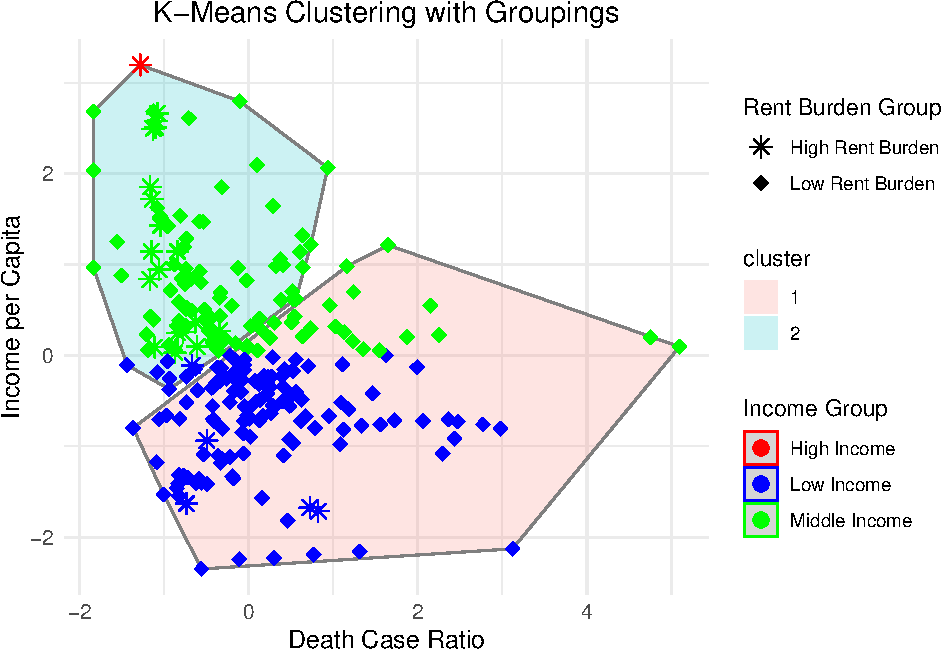
\includegraphics{Final-Report_files/figure-latex/supervised grouping on Cluster chart-1.pdf}
\captionof{figure}{K-Means Clustering with Groupings}

\vspace{10pt}

\textbf{Cluster 1 (Red Region)} This cluster is characterized by a
higher Death Case Ratio and generally lower ot middle Income per Capita.
The blue points represent low-income groups, and the density of these
points suggests a strong presence of economically vulnerable areas
within this cluster. The green points, representing middle-income
groups, are present but less dense compared to the low-income group.
Notably, this cluster contains both high and low rent burden subgroups,
with high rent burden subgroups (indicated by star-shaped markers) mixed
throughout. This implies that some areas within this cluster experience
compounded economic stress, both in terms of income and rent burden,
which could exacerbate health outcomes.

\vspace{5pt}

\textbf{Cluster 2 (Blue Region)} This cluster encompasses areas with a
lower Death Case Ratio and generally higher Income per Capita. The red
points indicate high-income areas, clustered toward the upper end of the
income per capita axis, reflecting wealthier regions with better
pandemic outcomes. There is a significant presence of green points
representing middle-income groups, indicating that this cluster captures
a range of moderately affluent areas. These areas seem to have fared
better in terms of health outcomes compared to Cluster 1. High-income
areas (red points) appear to have a mix of high and low rent burden
groups, but even those with high rent burdens display relatively low
Death Case Ratios. This suggests that wealthier regions, even with high
rent burdens, may have had resources to mitigate the pandemic's effects.

\vspace{5pt}

The clustering highlights a strong correlation between income and health
resilience. Higher income per capita is associated with lower Death Case
Ratios, likely due to better access to healthcare, resources, and
infrastructure to manage health crises. Low-income areas, especially
those burdened by high housing costs, appear more vulnerable. The
presence of both low and high rent burden groups in Cluster 1 suggests
that financial strain could amplify the negative impact of the pandemic.
Middle-income areas straddle both clusters, indicating that not all
middle-income regions experienced the pandemic uniformly. Factors beyond
income, such as healthcare infrastructure, population density, or social
support, could influence outcomes.

\vspace{5pt}

The following table presents the purity scores for the two different
subgroup classifications: Income Groups and Rent Burden Groups.

\begin{table}
\centering
\caption{\label{tab:purity calcuations}Purity Scores by Grouping}
\centering
\fontsize{10}{12}\selectfont
\begin{tabular}[t]{lr}
\toprule
Grouping & Purity\_Score\\
\midrule
Income Groups & 0.8700787\\
Rent Burden Groups & 0.9055118\\
\bottomrule
\end{tabular}
\end{table}

Purity is a metric used to evaluate the quality of clustering by
measuring the extent to which clusters contain data points of a single
class. A higher purity score indicates that the clusters are more
homogeneous concerning the given grouping.

\vspace{5pt}

\begin{itemize}
\tightlist
\item
  \textbf{Income:} A purity score of 0.870 indicates that 87.0 percent
  of the data points within clusters are correctly grouped based on
  their income level (Low, Middle, or High Income). The relatively high
  score suggests that the clustering model is effective in
  distinguishing counties based on income characteristics, but there is
  still a bit of overlap or misclassification. The presence of overlap
  could imply that income levels alone do not fully explain the
  clustering structure.
\item
  \textbf{Rent Burden:} The purity score for rent burden classification
  is 90.6 percent, which is slightly higher than the score for income
  groups. This suggests that the clusters are even better at grouping
  counties based on housing affordability stress, indicated by whether
  they experience high or low rent burdens. This could mean that rent
  burden is a more distinct factor in the clustering analysis.
\end{itemize}

\vspace{5pt}

Both scores are relatively high, indicating that the K-Means clustering
captures meaningful distinctions in the data. Given the high but not
perfect purity scores, there may be other unexamined variables
influencing the clusters. Additional socioeconomic or demographic
factors could be considered in future models to further refine the
clustering results. Overall, the analysis suggests that while both
income and rent burden are effective for understanding the clustering of
Texas counties, housing stress appears to be a particularly significant
and differentiating factor. This insight could be valuable for
stakeholders aiming to address economic disparities or plan for
community resilience.

\subsubsection{Heirarchical Clustering}\label{heirarchical-clustering}

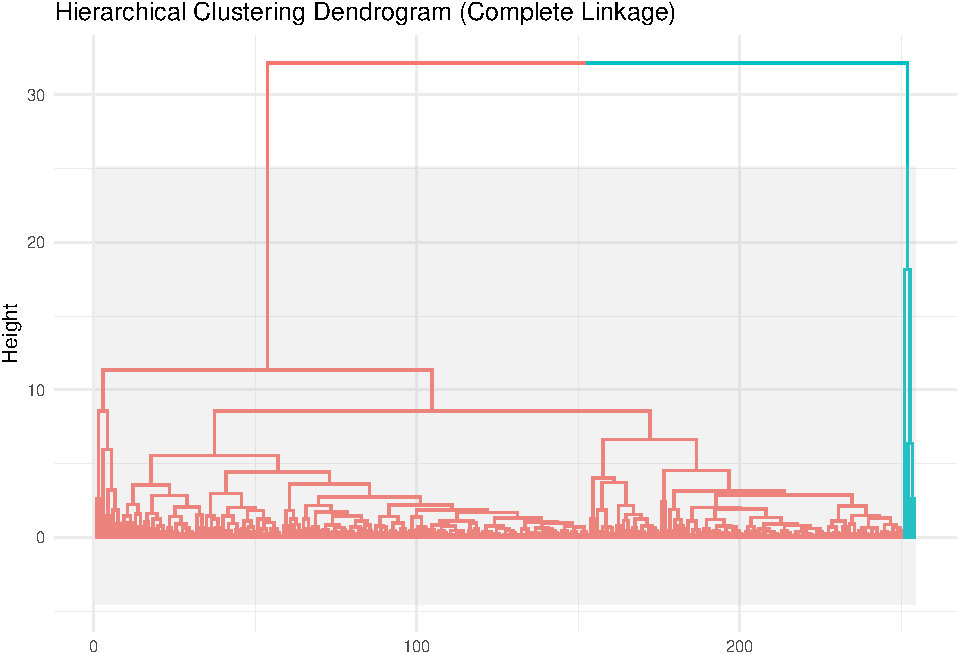
\includegraphics{Final-Report_files/figure-latex/hierarchical clustering-1.pdf}

\begin{table}[!h]
\centering
\caption{\label{tab:hierarchical summary}Summary Statistics by Hierarchical Cluster}
\centering
\fontsize{7}{9}\selectfont
\begin{tabular}[t]{>{\raggedright\arraybackslash}p{1.5cm}>{\raggedleft\arraybackslash}p{1.5cm}>{\raggedleft\arraybackslash}p{1.5cm}>{\raggedleft\arraybackslash}p{1.5cm}>{\raggedleft\arraybackslash}p{1.5cm}>{\raggedleft\arraybackslash}p{1.5cm}>{\raggedleft\arraybackslash}p{1.5cm}r}
\toprule
cluster\_hc & Avg
Median
Income & Avg
Income
per Capita & Avg
Rent
> 50\% & Avg
Rent
30-35\% & Avg
Confirmed
Cases & Avg
Deaths & Total
Population\\
\midrule
1 & 49780.86 & 24786.04 & 1551.7 & 615.408 & 5078.896 & 89.052 & 65864.8\\
2 & 56987.00 & 29420.25 & 91995.0 & 36522.250 & 217182.500 & 2529.000 & 2738352.8\\
\bottomrule
\end{tabular}
\end{table}

\paragraph{Suitable Number of
Clusters}\label{suitable-number-of-clusters-1}

The Elbow Method plots the WSS (Within-Cluster Sum of Squares) for
different number of clusters. WSS measures how tightly the data points
are grouped around the centroids of the clusters. After a certain point,
adding more clusters provides diminishing returns, meaning the reduction
in WSS becomes negligible. The optimal number of clusters is found at
the ``elbow'' point, where the rate of decrease in WSS sharply levels
off. In the following elbow plot, the elbow occurs around 2 clusters.
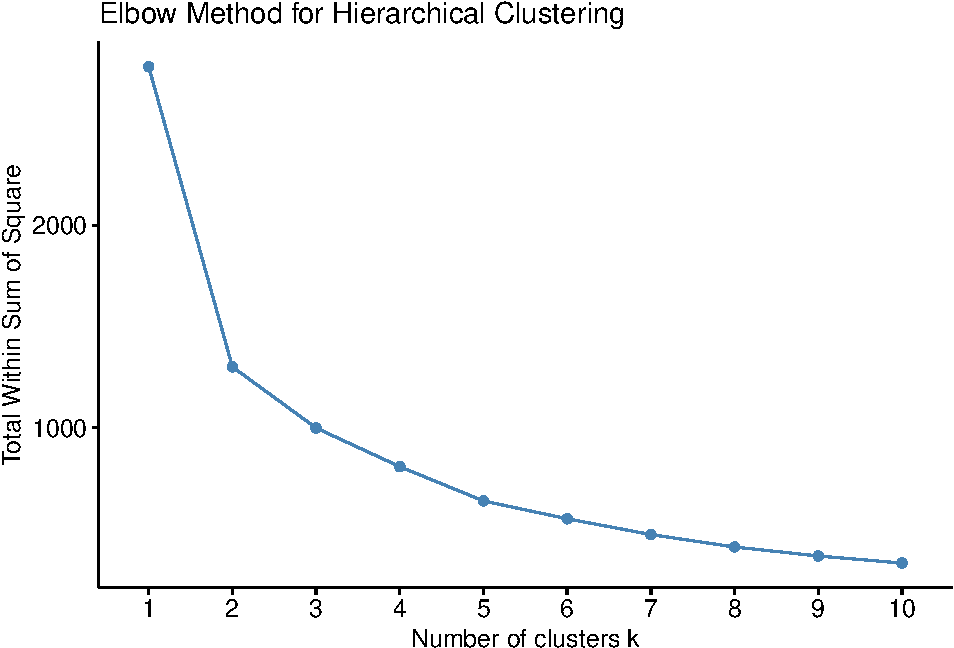
\includegraphics{Final-Report_files/figure-latex/heirarchical optimal cluster elbow-1.pdf}

The Silhouette Method evaluates how well each data point fits within its
assigned cluster compared to other clusters. The Silhouette score ranges
from -1 to 1, with values close to 1 meaning that the points are
well-clustered. In the following Silhouette chart, the peak occurs at 2
clusters.
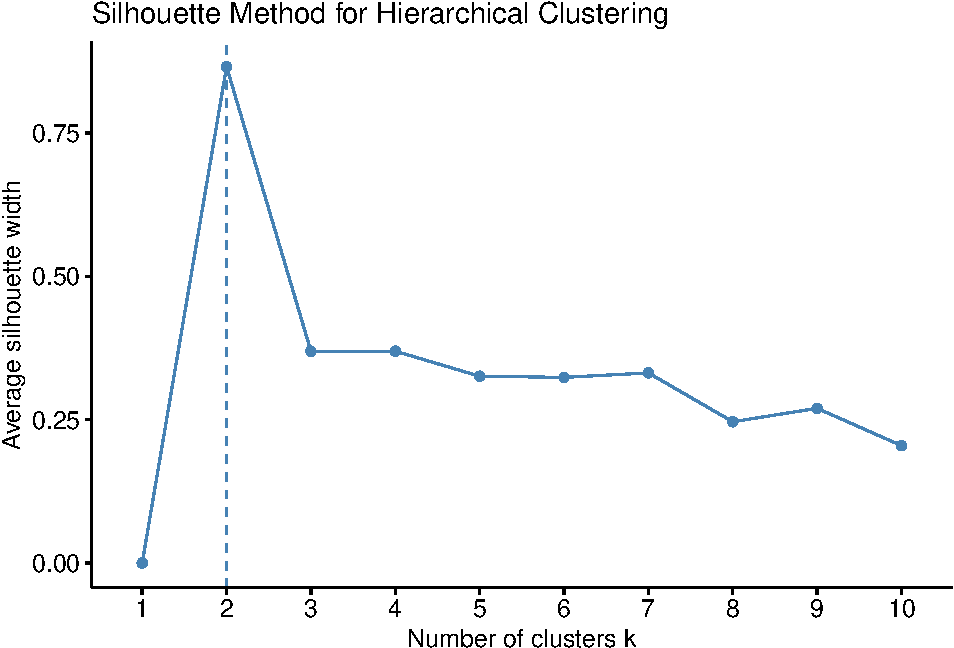
\includegraphics{Final-Report_files/figure-latex/heirarchical optimal cluster silhouette-1.pdf}

After considering both of these models, it was decided to do 2 clusters.
Because of the consistency across both methods, 2 cluters was the clear
choice.

\paragraph{Unsupervised Evaluation}\label{unsupervised-evaluation-1}

\begin{verbatim}
##   cluster size ave.sil.width
## 1       1  250          0.87
## 2       2    4          0.45
\end{verbatim}

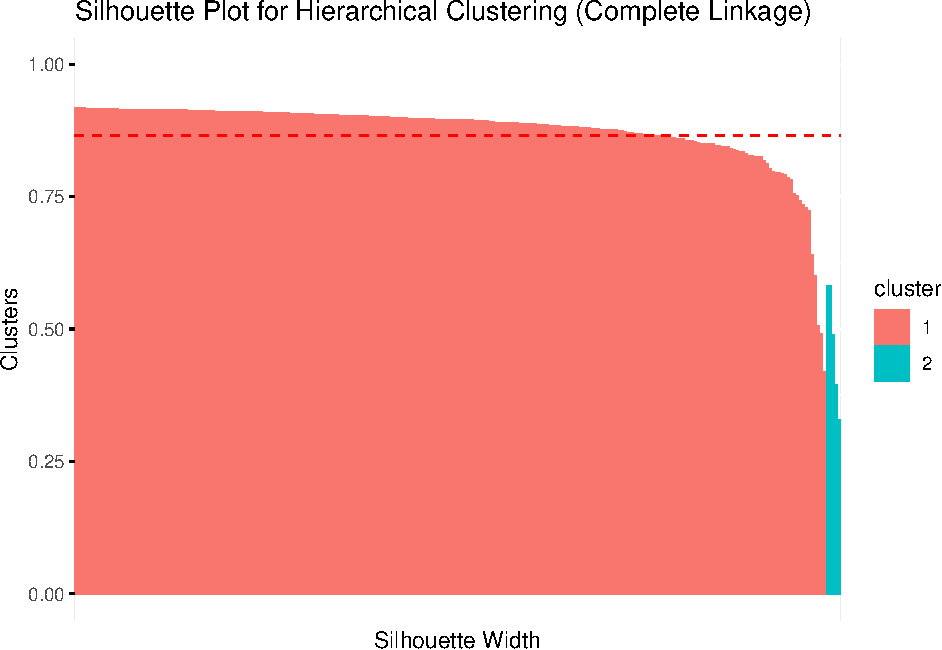
\includegraphics{Final-Report_files/figure-latex/hierarchical silhouette analysis-1.pdf}

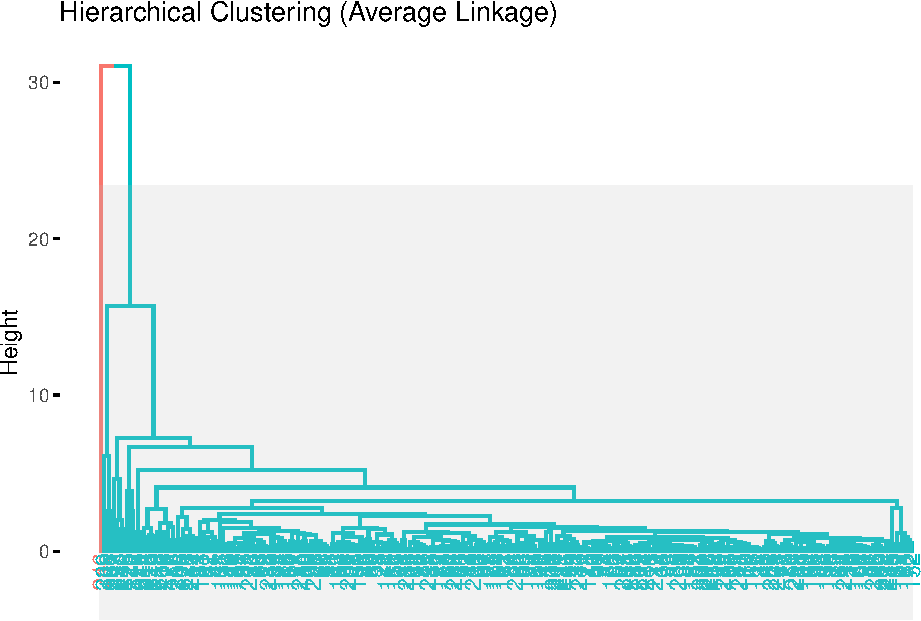
\includegraphics{Final-Report_files/figure-latex/hierarchical comaprison of linkage methods-1.pdf}
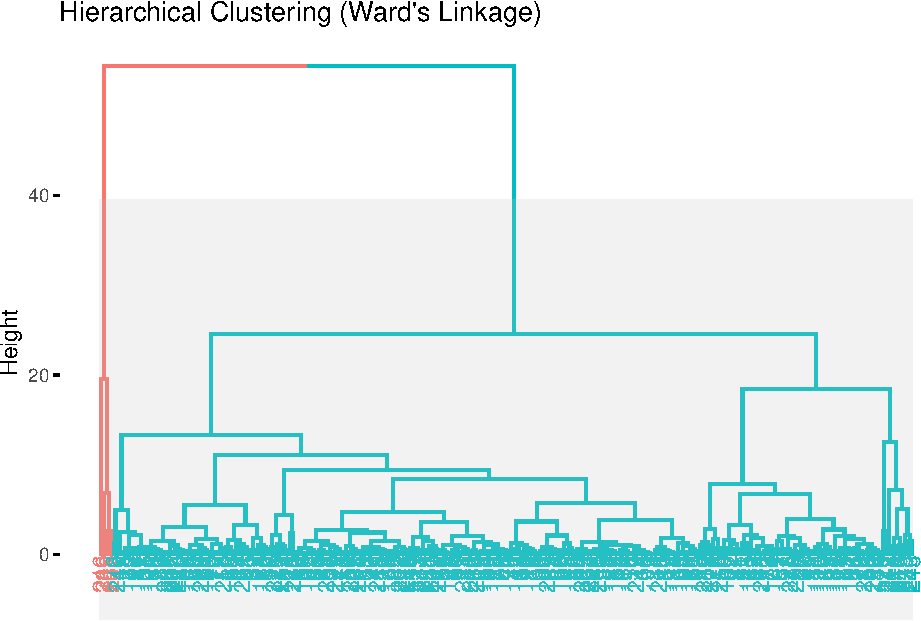
\includegraphics{Final-Report_files/figure-latex/hierarchical comaprison of linkage methods-2.pdf}

\begingroup\fontsize{8.5}{10.5}\selectfont

\begin{longtable}[t]{lr}
\caption{\label{tab:average silhouette width}Average Silhouette Widths by Linkage Method}\\
\toprule
Linkage\_Method & Avg\_Silhouette\_Width\\
\midrule
Complete & 1.984252\\
Average & 1.996063\\
Ward's & 1.984252\\
\bottomrule
\end{longtable}
\endgroup{}

\paragraph{Ground Truth Feature}\label{ground-truth-feature-1}

\begin{verbatim}
##    
##     Lower Higher
##   1   145    105
##   2     4      0
\end{verbatim}

\paragraph{Supervised Evaluation}\label{supervised-evaluation-1}

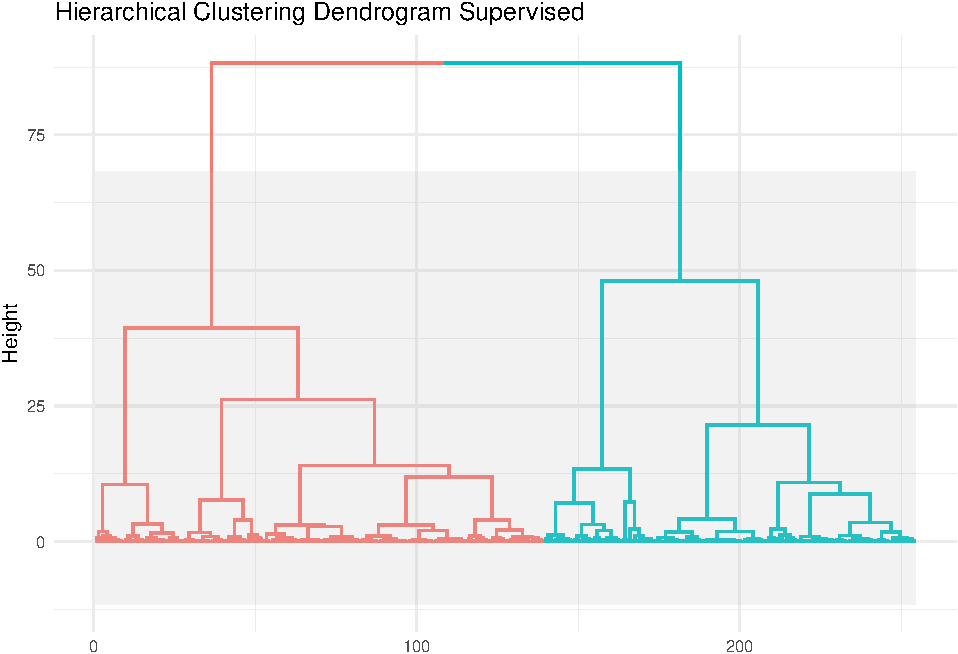
\includegraphics{Final-Report_files/figure-latex/hierarchical clustering supervised-1.pdf}

\begin{table}[!h]
\centering
\caption{\label{tab:hierarchical summary supervised}Summary Statistics by Hierarchical Cluster (Supervised)}
\centering
\fontsize{7}{9}\selectfont
\begin{tabular}[t]{>{\raggedright\arraybackslash}p{1.25 cm}>{\raggedleft\arraybackslash}p{1.25 cm}>{\raggedleft\arraybackslash}p{1.25 cm}>{\raggedleft\arraybackslash}p{1.25 cm}>{\raggedleft\arraybackslash}p{1.25 cm}>{\raggedleft\arraybackslash}p{1.25 cm}>{\raggedleft\arraybackslash}p{1.25 cm}>{\raggedleft\arraybackslash}p{1.25 cm}r}
\toprule
cluster\_hc & Avg
Median
Income & Avg
Income
per Capita & Avg
Rent
> 50\% & Avg
Rent
30-35\% & Avg
Confirmed
Cases & Avg
Deaths & Avg
Death Case Ratio & Total
Population\\
\midrule
1 & 42665.18 & 21229.01 & 829.9565 & 304.0609 & 3558.522 & 89.34783 & 0.0327401 & 39234.2\\
2 & 55875.29 & 27862.27 & 4751.5108 & 1906.2878 & 12440.460 & 159.02158 & 0.0180368 & 164803.4\\
\bottomrule
\end{tabular}
\end{table}

\newpage

\section{Population Data in Texas Counties/Layer 2
Clustering}\label{population-data-in-texas-countieslayer-2-clustering}

\subsection{Data Collection, Quality, and
Exploration}\label{data-collection-quality-and-exploration-1}

\subsubsection{Objects to Cluster}\label{objects-to-cluster-1}

The first part of the report clustered for the best performing affluent
counties using the death to cases ratio and income per capita. Our model
takes these optimal clusters of counties (cluster ``2'' in both
methodologies for prior layer of clustering) and applies a second layer
of clustering using the same methods.

That is to say, each methodology, K-means and Hierarchical, in this
second layer receives cluster ``2'' from its prior layer and applies
itself again (e.g.~The K-means method in this layer applies itself to
cluster ``2'' of the K-means result for death to cases ratio and income
per capita).

\subsubsection{Features for Clustering}\label{features-for-clustering-1}

The feature set for this second layer on which our K-means and
Hierarchical methods apply themselves are population density and
COVID-19 cases per thousand. This is done in order to find the highest
population density counties with the lowest amount of COVID-19 cases.

-\textbf{Population Density} Found by first obtaining the total
population for each Texas county using the Tidycensus R package, and
then using census.gov's 2023 Geographic info API to retrieve the
variable AREALAND\_SQMI (land area in square miles) for each county in
Texas. The total population for each county was divided by the total
land area in square miles to create the population density feature
(people per square mile of land). -\textbf{Cases per Thousand} Found by
taking total cases from COVID-19 Texas data set and dividing by total
population for each county.

\subsubsection{Table of Features and Basic
Statistics}\label{table-of-features-and-basic-statistics-1}

\begingroup\fontsize{10}{12}\selectfont

\begin{longtable}[t]{lllllll}
\caption{\label{tab:unnamed-chunk-4}Basic Statistics for Features}\\
\toprule
Feature & Min. & 1st Qu. & Median & Mean & 3rd Qu. & Max.\\
\midrule
Total Deaths & 0.00 & 14.00 & 32.00 & 135.35 & 84.75 & 4024.00\\
Total Cases & 1 & 505 & 1393 & 8854 & 3652 & 297629\\
Total Population & 117 & 6835 & 18522 & 112738 & 51864 & 4680609\\
Area in Square Miles & 127.2 & 835.7 & 908.7 & 1028.6 & 1043.4 & 6183.8\\
Population Density & 0.1749 & 6.3404 & 21.8211 & 119.3629 & 66.3361 & 3003.4746\\
\addlinespace
Deaths per Thousand & 0.000 & 1.227 & 1.781 & 1.960 & 2.542 & 5.838\\
Cases per Thousand & 8.547 & 60.369 & 78.495 & 80.639 & 97.758 & 179.111\\
\bottomrule
\end{longtable}
\endgroup{}

\subsubsection{Scale of Measurement}\label{scale-of-measurement-1}

\begingroup\fontsize{10}{12}\selectfont

\begin{longtable}[t]{lll}
\caption{\label{tab:unnamed-chunk-5}Measurement Scales for Features}\\
\toprule
Features & Scale & Description\\
\midrule
County Name & Nominal & Name of the county\\
Total Deaths & Ratio & Total Amount of Deaths in the County\\
Total Cases & Ratio & Total Amount of Cases in the County\\
Total Population & Ratio & Total Population of the County\\
Area in Square Miles & Ratio & Area of county in Square Miles\\
\addlinespace
Population Density & Ratio & Population Density in People per Square Mile\\
Deaths per Thousand & Ratio & Covid Deaths per Thousand Inhabitants\\
Cases per Thousand & Ratio & Covid Cases per Thousand Inhabitants\\
\bottomrule
\end{longtable}
\endgroup{}

\subsubsection{Measures for
Similarity/Distance}\label{measures-for-similaritydistance-1}

Since the clustering uses K-means and Hierarchical methodologies,
Euclidean distance is used. Here are
first-five-counties-in-the-data-set's euclidean distance for population
density and cases per thousand.

\begin{verbatim}
##           1         2         3         4
## 2 98.126290                              
## 3  6.201082 97.470224                    
## 4 29.604521 70.963217 31.467442          
## 5 52.011261 51.166822 49.634707 33.772758
\end{verbatim}

\subsubsection{Normalization/Standardization}\label{normalizationstandardization-1}

Numeric features in the data set were normalized using R's scale
function, which normalizes a distribution using a standard Z-score
normalization.

\subsection{Modeling and Evaluation}\label{modeling-and-evaluation-1}

\subsubsection{K-Means Clustering}\label{k-means-clustering-1}

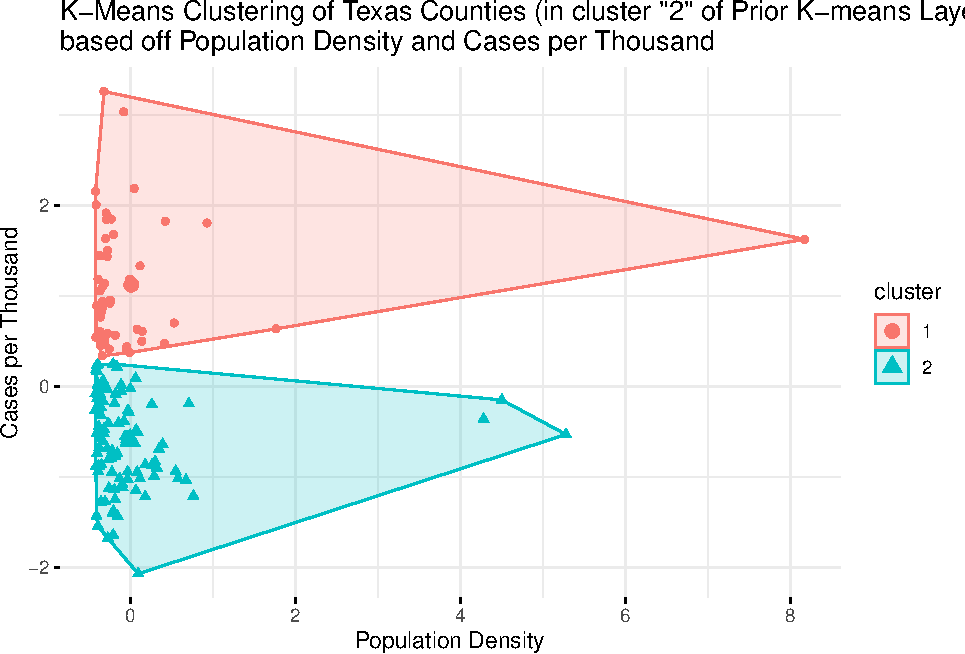
\includegraphics{Final-Report_files/figure-latex/unnamed-chunk-8-1.pdf}

Our K-means clustering seemingly divides the data into low
cases-per-thousand and high cases-per-thousand.

\paragraph{Suitable Number of
Clusters}\label{suitable-number-of-clusters-2}

Elbow Method

\begin{verbatim}
## Warning: Using `size` aesthetic for lines was deprecated in ggplot2 3.4.0.
## i Please use `linewidth` instead.
## This warning is displayed once every 8 hours.
## Call `lifecycle::last_lifecycle_warnings()` to see where this warning was
## generated.
\end{verbatim}

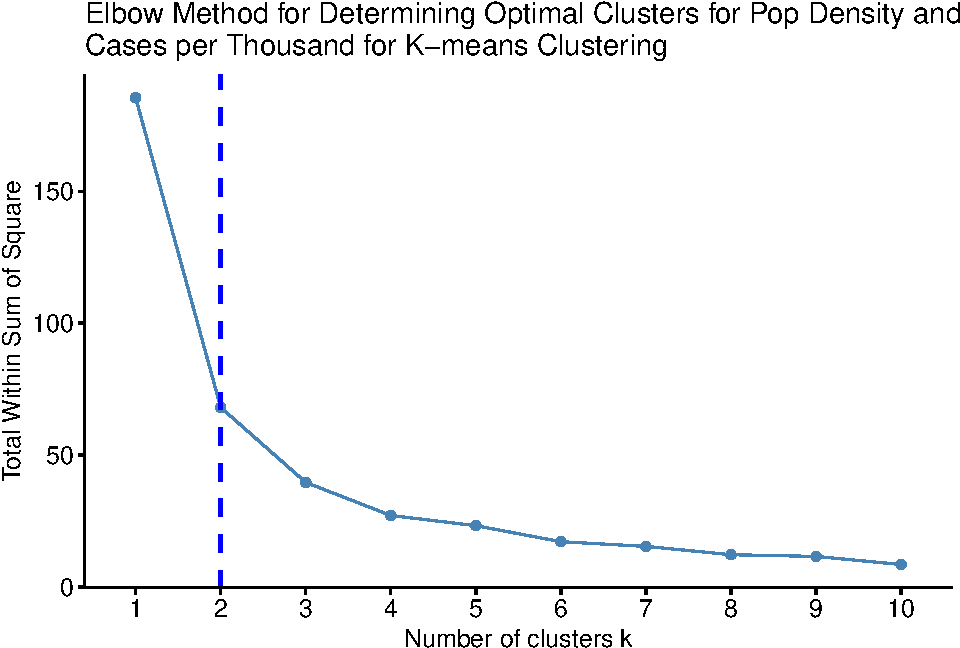
\includegraphics{Final-Report_files/figure-latex/unnamed-chunk-10-1.pdf}

Silhouette Method

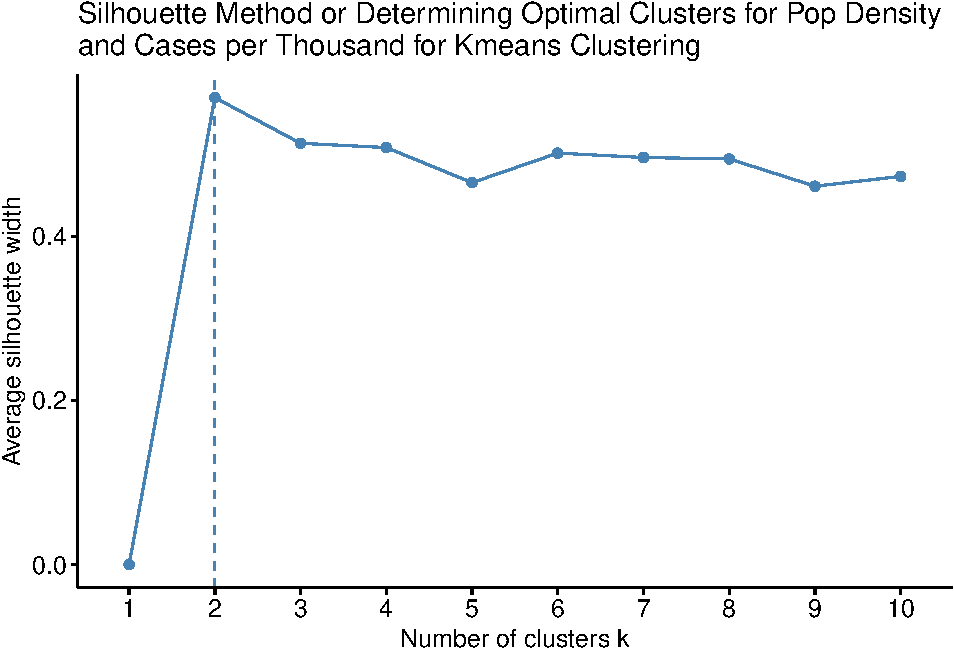
\includegraphics{Final-Report_files/figure-latex/unnamed-chunk-11-1.pdf}

Our Elbow and Silhouette methods suggest our optimal amount of clusters
for K-means is 2 clusters.

\paragraph{Unsupervised Evaluation}\label{unsupervised-evaluation-2}

Silhouette Width

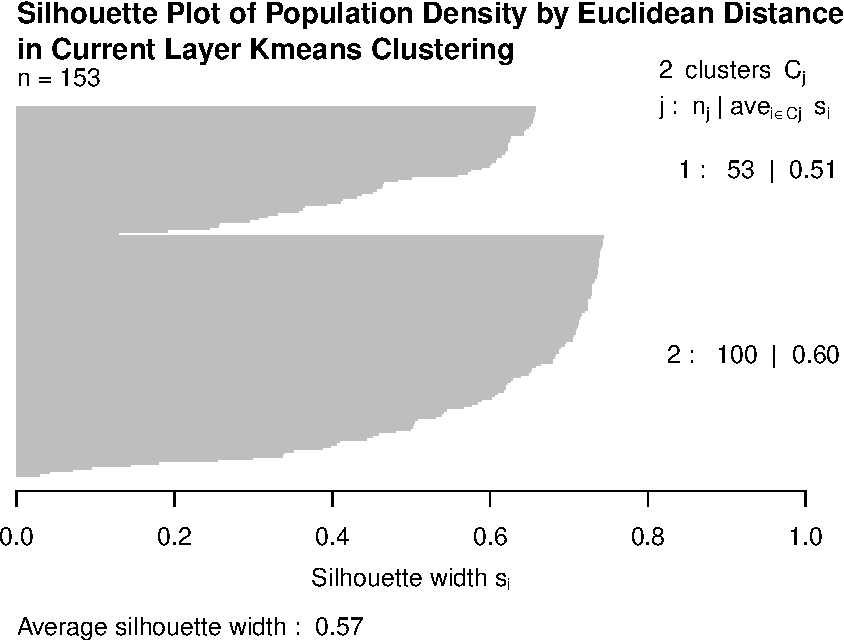
\includegraphics{Final-Report_files/figure-latex/unnamed-chunk-13-1.pdf}

Our Average Silhouette width is not close to 1, which means that the
centroids may not be as close to the middle of the cluster as they could
be; however, the distribution of data points are fair.

Summary Statistics

\begin{table}[!h]
\centering
\caption{\label{tab:unnamed-chunk-14}Summary Statistics for K-means Cluster based on Population Density and Cases per Thousand}
\centering
\fontsize{7}{9}\selectfont
\begin{tabular}[t]{>{\raggedright\arraybackslash}p{1.25 cm}>{\raggedleft\arraybackslash}p{1.25 cm}>{\raggedleft\arraybackslash}p{1.25 cm}>{\raggedleft\arraybackslash}p{1.25 cm}>{\raggedleft\arraybackslash}p{1.25 cm}>{}p{1.25 cm}>{}p{1.25 cm}>{}p{1.25 cm}}
\toprule
layer\_2\_kmeans & Avg
Cases
per
thousand & Avg
Deaths
per
thousand & Avg
Population
Density & Number
of
Counties\\
\midrule
1 & 116.9643 & 2.809818 & 42.08026 & 53\\
2 & 66.9696 & 2.213788 & 40.84501 & 100\\
\bottomrule
\end{tabular}
\end{table}

As mentioned earlier, the second layer of K-means clustering seemingly
prioritized cases-per-thousands over population density.

\paragraph{Ground Truth Feature}\label{ground-truth-feature-2}

\paragraph{Supervised Evaluation}\label{supervised-evaluation-2}

\subsubsection{Heirarchical Clustering}\label{heirarchical-clustering-1}

Dendogram

\begin{verbatim}
## Warning in dist(counties_hierarchical_pop_dens_et_cases_per_k.scaled): NAs
## introduced by coercion
\end{verbatim}

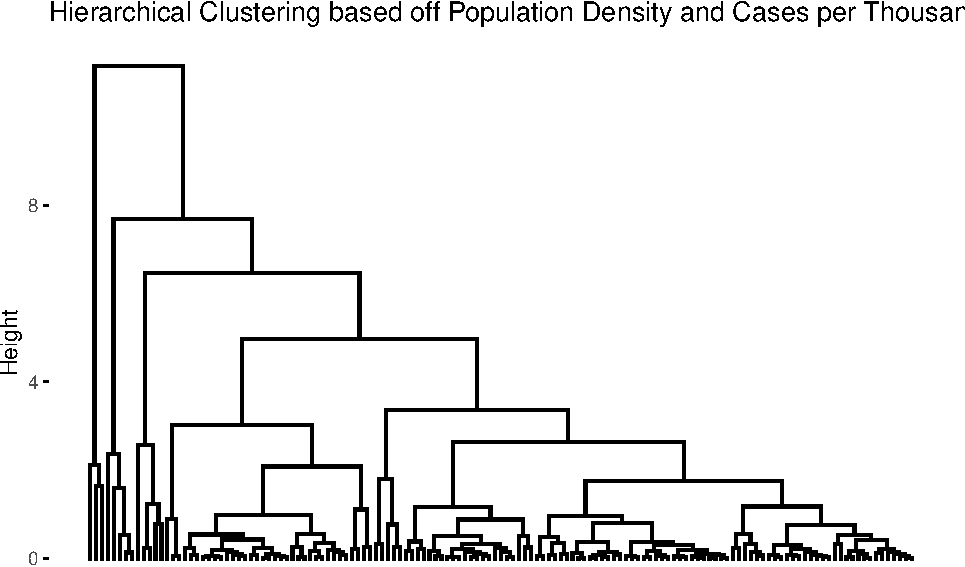
\includegraphics{Final-Report_files/figure-latex/unnamed-chunk-16-1.pdf}

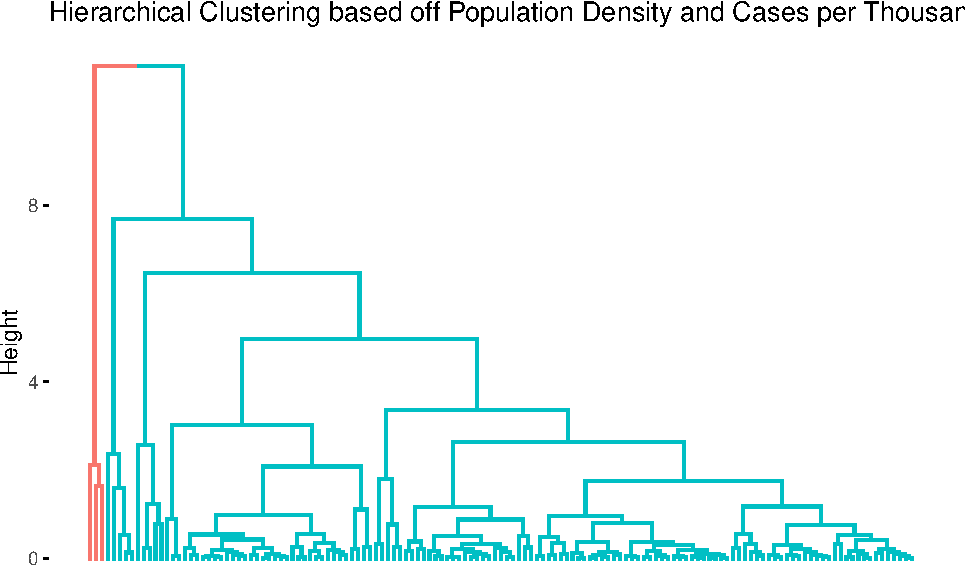
\includegraphics{Final-Report_files/figure-latex/unnamed-chunk-17-1.pdf}

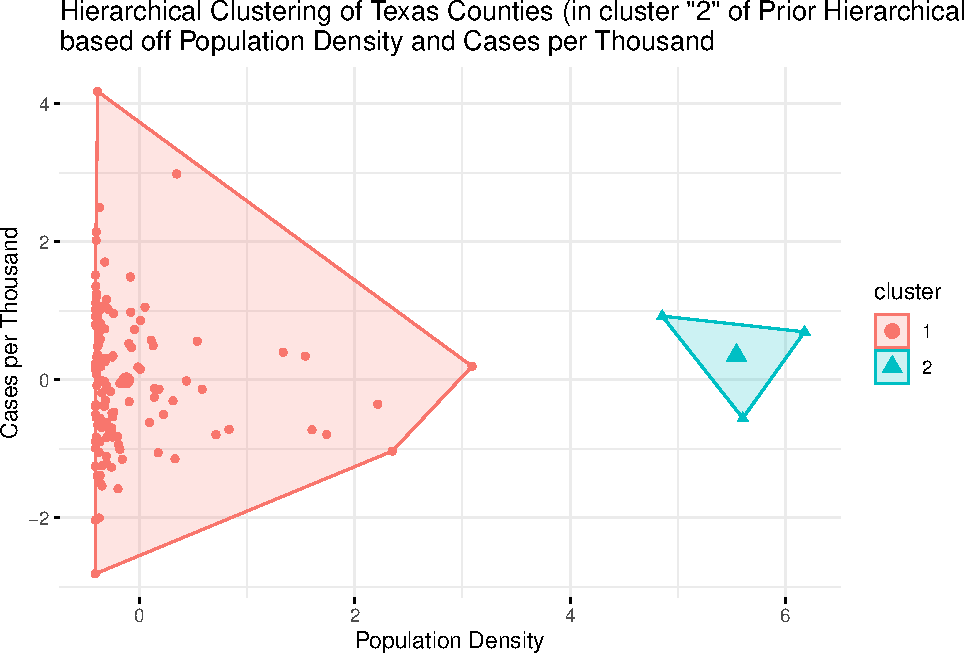
\includegraphics{Final-Report_files/figure-latex/unnamed-chunk-18-1.pdf}

The second layer Hierarchical clustering seemingly divides the data into
high and low population density.

\paragraph{Suitable Number of
Clusters}\label{suitable-number-of-clusters-3}

Elbow

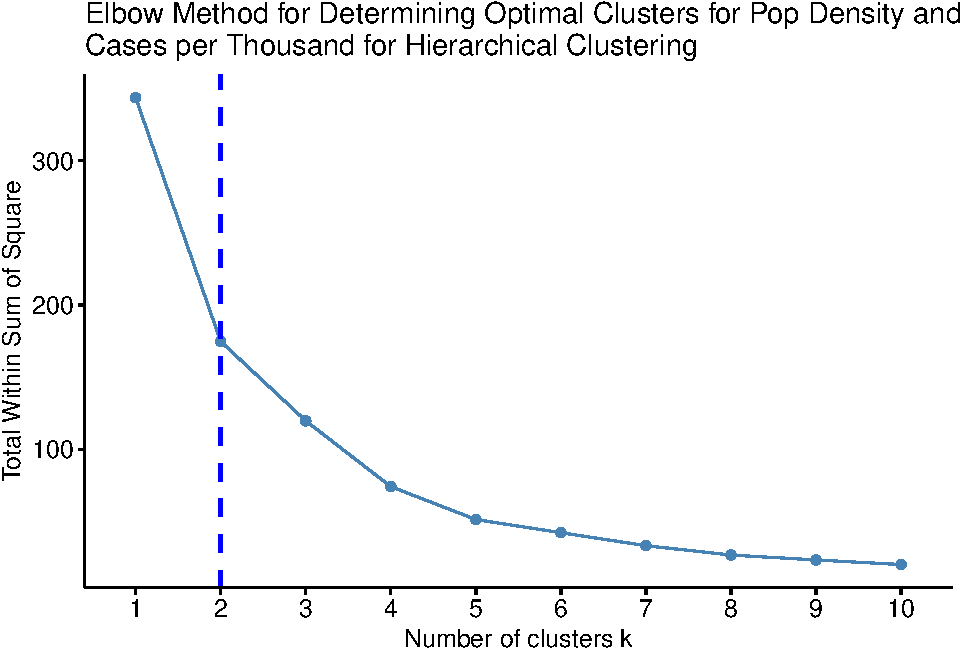
\includegraphics{Final-Report_files/figure-latex/unnamed-chunk-19-1.pdf}

Silhouette Method

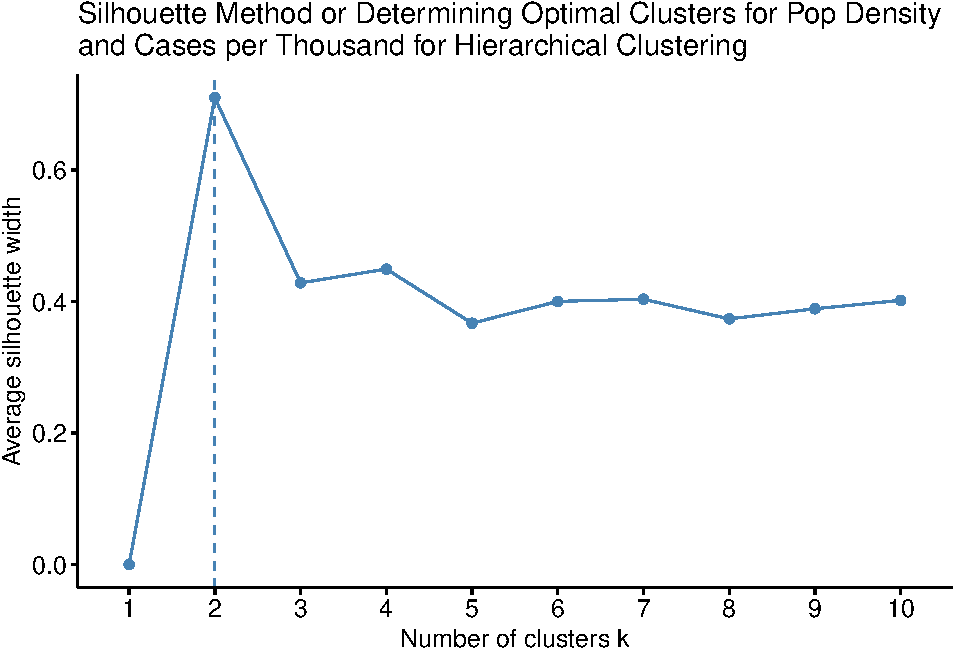
\includegraphics{Final-Report_files/figure-latex/unnamed-chunk-20-1.pdf}

Our Elbow and Silhouette methods suggest our Hierarchical Dendogram be
cut at 2 clusters.

\paragraph{Unsupervised Evaluation}\label{unsupervised-evaluation-3}

Silhouette Plot

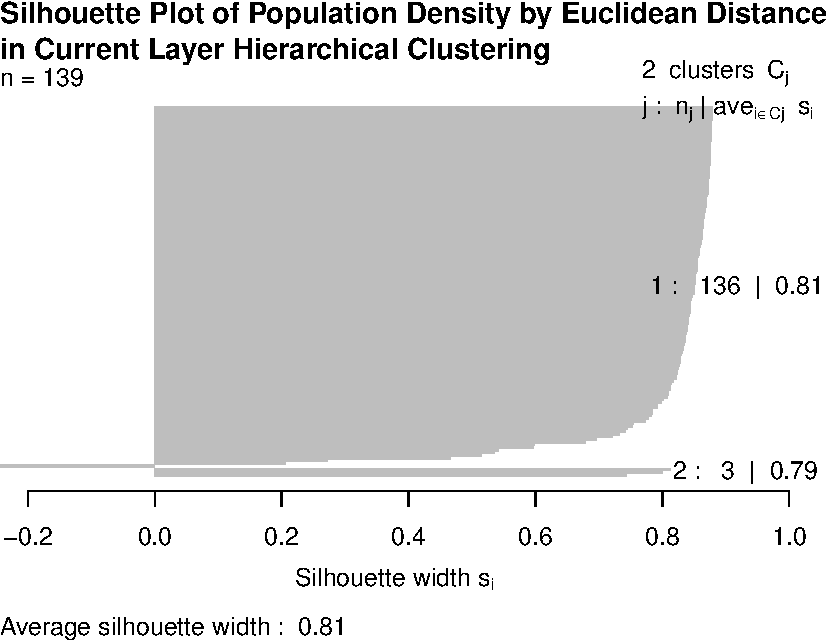
\includegraphics{Final-Report_files/figure-latex/unnamed-chunk-22-1.pdf}

Our average silhouette widths are close to 1, which means the centroids
are close to the center of the clusters; however, the distribution of
data points in the cluster are very lop sided in favor of the low
population density cluster.

Summary Statistics

\begin{table}[!h]
\centering
\caption{\label{tab:unnamed-chunk-23}Summary Statistics for Hierarchical Cluster based on Population Density and Cases per Thousand}
\centering
\fontsize{7}{9}\selectfont
\begin{tabular}[t]{>{\raggedleft\arraybackslash}p{1.25 cm}>{\raggedleft\arraybackslash}p{1.25 cm}>{\raggedleft\arraybackslash}p{1.25 cm}>{\raggedleft\arraybackslash}p{1.25 cm}>{\raggedleft\arraybackslash}p{1.25 cm}>{}p{1.25 cm}>{}p{1.25 cm}>{}p{1.25 cm}}
\toprule
layer\_2\_hierarchical & Avg
Cases
per
thousand & Avg
Deaths
per
thousand & Avg
Population
Density & Number
of
Counties\\
\midrule
1 & 76.95841 & 1.426565 & 130.5207 & 136\\
2 & 85.79536 & 0.934339 & 2715.3660 & 3\\
\bottomrule
\end{tabular}
\end{table}

As mentioned earlier, the distribution of number of counties in a
cluster could be better; however, the three counties found in the second
county have a notably low deaths per thousand despite clustering for
cases per thousand.

\paragraph{Ground Truth Feature}\label{ground-truth-feature-3}

\paragraph{Supervised Evaluation}\label{supervised-evaluation-3}

\newpage

\section{Exceptional Work}\label{exceptional-work}

\subsection{Data Collection, Quality, and
Exploration}\label{data-collection-quality-and-exploration-2}

\subsubsection{Objects to Cluster}\label{objects-to-cluster-2}

\subsubsection{Features for Clustering}\label{features-for-clustering-2}

\subsubsection{Table of Features and Basic
Statistics}\label{table-of-features-and-basic-statistics-2}

\subsubsection{Scale of Measurement}\label{scale-of-measurement-2}

\subsubsection{Measures for
Similarity/Distance}\label{measures-for-similaritydistance-2}

\subsubsection{Normalization/Standardization}\label{normalizationstandardization-2}

\subsection{Modeling and Evaluation}\label{modeling-and-evaluation-2}

\subsubsection{Clustering \_\_\_\_\_}\label{clustering-_____}

\paragraph{Suitable Number of
Clusters}\label{suitable-number-of-clusters-4}

\paragraph{Unsupervised Evaluation}\label{unsupervised-evaluation-4}

\paragraph{Ground Truth Feature}\label{ground-truth-feature-4}

\paragraph{Supervised Evaluation}\label{supervised-evaluation-4}

\subsubsection{Clustering \_\_\_\_\_\_}\label{clustering-______}

\paragraph{Suitable Number of
Clusters}\label{suitable-number-of-clusters-5}

\paragraph{Unsupervised Evaluation}\label{unsupervised-evaluation-5}

\paragraph{Ground Truth Feature}\label{ground-truth-feature-5}

\paragraph{Supervised Evaluation}\label{supervised-evaluation-5}

\newpage

\section{Recommendations}\label{recommendations}

\emph{Discuss how the model can be interpreted and the recommendations
based on the findings. Explain the utility for the stakeholders.}

After analyzing our model's results, if a client has an interest in
opening a business in an affluent, high land population density, and
high COVID-19 performing county in Texas, they should consider the
following counties.

After taking cluster ``1'' in the second layer K-means cluster, and
sorting from descending order according to population density the three
top counties are:

\begin{table}[!h]
\centering
\caption{\label{tab:unnamed-chunk-24}Summary Statistics by Cluster}
\centering
\fontsize{7}{9}\selectfont
\begin{tabular}[t]{>{\raggedright\arraybackslash}p{1.25 cm}>{}p{1.25 cm}>{}p{1.25 cm}>{}p{1.25 cm}>{}p{1.25 cm}>{}p{1.25 cm}>{}p{1.25 cm}>{}p{1.25 cm}}
\toprule
county\_name\\
\midrule
El Paso County\\
Wichita County\\
Potter County\\
\bottomrule
\end{tabular}
\end{table}

The three results in cluster ``2'' for the second layer hierarchical
clustering were:

\begin{table}[!h]
\centering
\caption{\label{tab:unnamed-chunk-25}Summary Statistics by Cluster}
\centering
\fontsize{7}{9}\selectfont
\begin{tabular}[t]{>{\raggedright\arraybackslash}p{1.25 cm}>{}p{1.25 cm}>{}p{1.25 cm}>{}p{1.25 cm}>{}p{1.25 cm}>{}p{1.25 cm}>{}p{1.25 cm}>{}p{1.25 cm}}
\toprule
county\_name\\
\midrule
Dallas County\\
Harris County\\
Tarrant County\\
\bottomrule
\end{tabular}
\end{table}

\begin{verbatim}
## Joining with `by = join_by(county_name)`
\end{verbatim}

\begin{table}[!h]
\centering
\caption{\label{tab:unnamed-chunk-26}Summary Statistics by Cluster}
\centering
\fontsize{7}{9}\selectfont
\begin{tabular}[t]{>{\raggedright\arraybackslash}p{1.25 cm}>{\raggedleft\arraybackslash}p{1.25 cm}>{\raggedleft\arraybackslash}p{1.25 cm}>{\raggedleft\arraybackslash}p{1.25 cm}>{\raggedleft\arraybackslash}p{1.25 cm}>{\raggedleft\arraybackslash}p{1.25 cm}>{\raggedleft\arraybackslash}p{1.25 cm}>{\raggedleft\arraybackslash}p{1.25 cm}rrrr}
\toprule
County
Name & Total
Population & Median
Income & Income
Per
Capita & Rent
Over
50\% & Rent
30-35\% & Confirmed
Cases & Confirmed
Deaths & Cases
per
Thousand & Deaths
Per
Thousand & Death
Case
Ratio & Population
Density\\
\midrule
Dallas County & 2552213 & 53626 & 29810 & 95830 & 38717 & 234625 & 2453 & 94.11149 & 1.0054777 & 0.0104550 & 3003.4746\\
Harris County & 4525519 & 57791 & 30856 & 158668 & 61305 & 286356 & 3825 & 63.58767 & 0.8597172 & 0.0133575 & 2741.9815\\
Tarrant County & 1983675 & 62532 & 30857 & 56570 & 24381 & 195518 & 1798 & 99.68693 & 0.9378221 & 0.0091961 & 2400.6419\\
El Paso County & 834825 & 43244 & 19950 & 19775 & 9431 & 107552 & 1940 & 131.58445 & 2.4662003 & 0.0180378 & 825.7745\\
Wichita County & 131778 & 45776 & 23263 & 4295 & 1618 & 13325 & 260 & 102.79674 & 2.1414410 & 0.0195122 & 210.5728\\
\addlinespace
Potter County & 121230 & 41852 & 21941 & 4276 & 1371 & 15947 & 302 & 136.81195 & 2.6875586 & 0.0189377 & 130.2557\\
\bottomrule
\end{tabular}
\end{table}

\emph{Describe your results. What recommendations can you formulate
based on the clustering results? How do these recommendations relate to
the ones already presented in report 1? What findings are the most
interesting to your stakeholder?}

\newpage

\section{Conclusion}\label{conclusion}

\emph{Summarize the key findings and their relevance to the initial
questions.}

\newpage

\section{List of References}\label{list-of-references}

{[}1{]} ``Covid-19,'' NFID,
\url{https://www.nfid.org/infectious-diseases/covid-19/} (accessed
Oct.~8, 2024).

{[}2{]} Northwestern Medicine, ``Covid-19 pandemic timeline,''
Northwestern Medicine,
\url{https://www.nm.org/healthbeat/medical-advances/new-therapies-and-drug-trials/covid-19-pandemic-timeline}
(accessed Oct.~8, 2024).

{[}3{]} ``10.1 - hierarchical clustering,'' 10.1 - Hierarchical
Clustering \textbar{} STAT 555,
\url{https://online.stat.psu.edu/stat555/node/85/\#:~:text=For\%20most\%20common\%20hierarchical\%20clustering,when\%20they\%20are\%20perfectly\%20correlated.}
(accessed Oct.~23, 2024).

{[}4{]} ``Manhattan distance,'' Wikipedia,
\url{https://simple.wikipedia.org/wiki/Manhattan_distance} (accessed
Oct.~23, 2024).

{[}5{]} A. Jain, ``Normalization and standardization of Data,''
Medium,\\
\href{https://medium.com/@abhishekjainindore24/normalization-and-standardization-of-data-408810a88307}{https://medium.com/@abhishekjainindore24/normalization-and-standardization-of-data-408810a88307}
(accessed Oct.~23, 2024).

\newpage

\section{Appendix}\label{appendix}

\emph{Include code snippets, extended tables, or other supplementary
information.}

\subsection{Student Contributions}\label{student-contributions}

Olivia Hofmann

\begin{itemize}
\tightlist
\item
  Format/Organization of Report (Lead)
\item
  Problem Description (Lead)
\item
  Income Data in Texas Counties (Lead)
\item
  Exceptional Work (Supporter)
\end{itemize}

Mike Perkins

\begin{itemize}
\tightlist
\item
  Format/Organization of Report (Supporter)
\item
  Exceptional Work (Lead)
\end{itemize}

Matias Barcelo

\begin{itemize}
\tightlist
\item
  Format/Organization of Report (Supporter)
\item
  Population Data in Texas Counties (Lead)
\end{itemize}

\subsection{Extra Graduate Student
Work}\label{extra-graduate-student-work}

\emph{For each graduate students: Describe your exceptional work in a
few sentences.}

The graduate students in this group are Olivia Hofmann and Mike Perkins.
Both graduate students worked together to ensure the report was held to
a high standard and complete the exceptional work clustering.

\end{document}
